\documentclass{article}
\usepackage[utf8]{inputenc}
\usepackage{adjustbox}
\usepackage{float}

%\title{Starcraft II for Multivariate Statistical Analysis}
\begin{document}
\begin{titlepage}
\begin{center}
\vspace*{1cm}
 
\huge
\textbf{Predicting player's leagues in Starcraft II}
 
\vspace{2cm}
Project Work for Multivariate Statistical Analysis
 
\vspace{1cm}
 
\textbf{Ari-Pekka Härkönen}
       
591881



8.4.2019
\vfill
 
\vspace{0.8cm}
 
\end{center}
\end{titlepage}

%\begin{document}

\section{Introduction}
Starcraft II is a real-time strategy (RTS) game developed by Blizzard Entertainment. The original game, Starcraft II Wings of Liberty, was released in 2010 and since then it has been expanded with two releases, Heart of the Swarm in 2013 and Legacy of the Void in 2015. The game is still widely popular around the world and has developed a large and active E-sports scene, with the prizes of the the top tournaments consisting of hundreds of thousands of US dollars. Watching the game is an especially popular past time in South Korea, which has no doubt contributed into most of the top players coming from there. In fact, the top competitive league of Starcraft II, World Championship Series, has been always won by a Korean player, except for 2018 when it was won by Joona "Serral" Sotala.

In my project, I wanted to examine how well a player's ranking in Starcraft II can be predicted by analyzing their in-game behavior. To predict a player's league, a dataset of previous game replays is analyzed. The research questions tackled in this project are related to performing this analysis with the mentioned observability requirement. More specifically, the research questions considered are:

\begin{itemize}
    \item Can a player's league be predicted by observing their in-game behaviour?
    \item Which variables of the used dataset provide the best clues for the league a player belongs to?
    \item How accurately can a players league be predicted by performing analysis on this dataset?
\end{itemize}

As an additional requirement, the variables that we consider are observable to any watcher of any game of Starcraft II. This allows anyone to utilize the results of this project to have an educated guess of a players league by observing the amount to which they correspond with the key variables introduced later.

\subsection{Dataset}
The dataset used in this statistical analysis is Starcraft II Replay Analysis found in Kaggle (\url{https://www.kaggle.com/sfu-summit/starcraft-ii-replay-analysis}). The original dataset contains observations from 3395 Starcraft II games with 21 variables describing the player behaviour. For the analysis performed here, we focus on a subset of 4 variables. The two main reasons for this are firstly the redundancy of some of the variables included in the set, the variables that are left out of this analysis measure behavior only visible to the player alone and using those to predict a player's success in the game is impossible as the data is not accessible until after the game. The second reason for the exclusion of some of the variables is that they do not clearly relate to a player's success or they are already presented by other variables in the dataset.

Below are introduced the variables included in this analysis. The decision of which variables from the original dataset are included and which are left out is based on my excessive knowledge of the game gained over years of trying to get out of Bronze league. With my expertise, I have chosen variables that are easily observed when watching a game and that represent different aspects of in-game strategies. Additionally, I wanted to keep the amount of variables low for the sake of fitting this report into ten pages. The next sections introduce the included variables. Table 1 shows the means and variances of each variable.

\begin{center}
\begin{tabular} { | c | c | c | c | c | }
\hline
Variable & League & APM & Selections by hotkey & Complex ability used \\
\hline
Mean & 4.10 & 117.0 & 0.00429 & 0.000142 \\
\hline
Variance & 2.30 & 2700.0 & 0.0000279 & 7.04e-08 \\
\hline
\end{tabular}
\caption{Table 1: means and variances of each variable}
\label{table:1}
\end{center}

\subsubsection{League}
League of a player is the basic measure for how good a player is in competitive Starcraft. By playing well enough, a player can advance to the next league. There are seven leagues in total: Bronze, Silver, Gold, Diamond, Master, GrandMaster and professional leagues. The professional leagues are additionally divided into two, but for the sake of simplicity the professionals are kept as one group. Figure 1 shows how the players in the dataset are distributed over different leagues.

\begin{figure} [H]
    \centering
    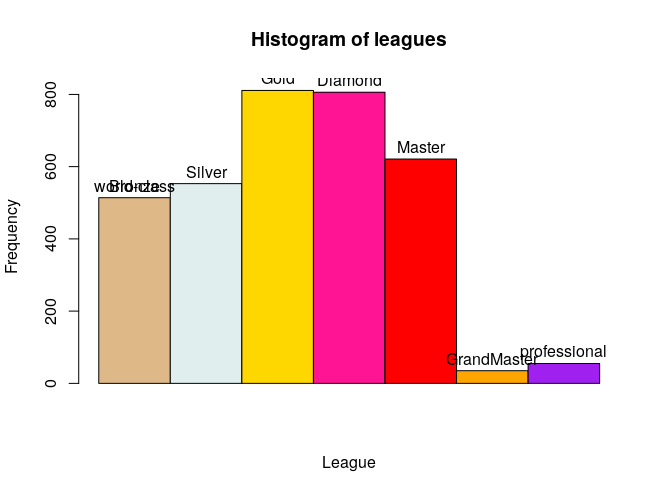
\includegraphics[width= 0.8\textwidth]{league_hist.png}
    \label{figure:league-hist}
    \caption{This histogram presents the distribution of leagues over the observations in the dataset.}
\end{figure}

\subsubsection{Actions Per Minute}
Actions per minute (APM) is a measure used in RTS-games to determine how much a player can get done in a given timespan. The APM value is an integer that corresponds with how many actions (clicks, or button presses) a player performs in one minute of game time. This can range anywhere from zero (player does nothing during a game) to well over 300 in the professional league. In the dataset used for this project, the smallest APM recorded is 22.0, while the largest is 389.8.

\begin{figure} [H]
    \centering
    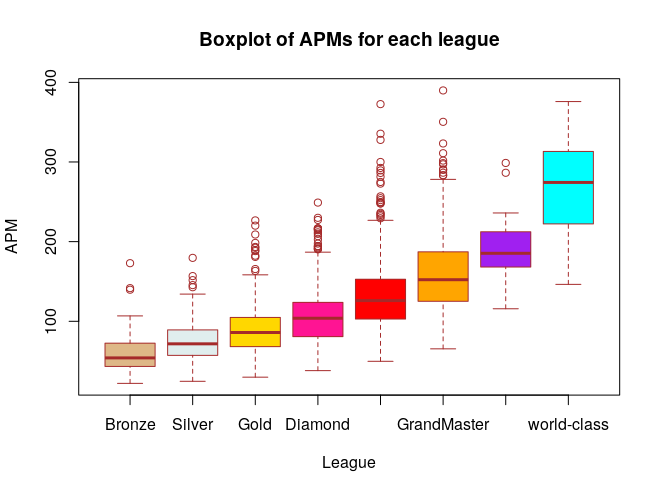
\includegraphics[width=0.8\textwidth]{apm_boxplot.png}
    \label{figure:figure:apm-boxplot}
    \caption{This figure shows how the APMs are distributed in each league.}
\end{figure}

As can be seen from the figure above, the APM among the players steadily rises as the leagues get more prestigious. It can be hard to determine the specific league of a player by knowing their APM, but an educated guess should hit the right ballpark, although as can be seen, there are some outliers in the data.

\subsubsection{Select by Hotkeys}
A hotkey references to a shortcut to an action by pressing a key in the keyboard. In Starcraft II players are allowed to place up to 10 units or groups of units (units are controllable characters) selectable by different hotkeys, which makes controlling those units a lot easier in complex situations and large battles. In the dataset used, the select by hotkeys -variable is the amount of selections made by a player using those hotkeys per timestamp in a game.

\begin{figure} [H]
    \centering
    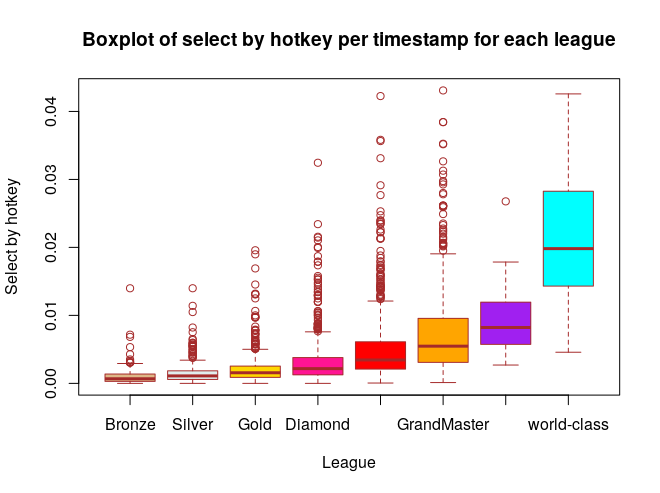
\includegraphics[width=0.8\textwidth]{hotkey_boxplot.png}
    \label{figure:figure:hotkey-boxplot}
    \caption{This figure shows how often players in each league use selection by hotkeys.}
\end{figure}

\subsubsection{Complex Abilities Used}
Starcraft II has many player controllable units, and many of those units have unique abilities that the players can utilize. These can be called by the player, but require the unit to be selected and a target to be chosen, which can be quite a hassle if the player is in a battle situation since the time used to assign an ability could be used to place many other moves.

\begin{figure} [H]
    \centering
    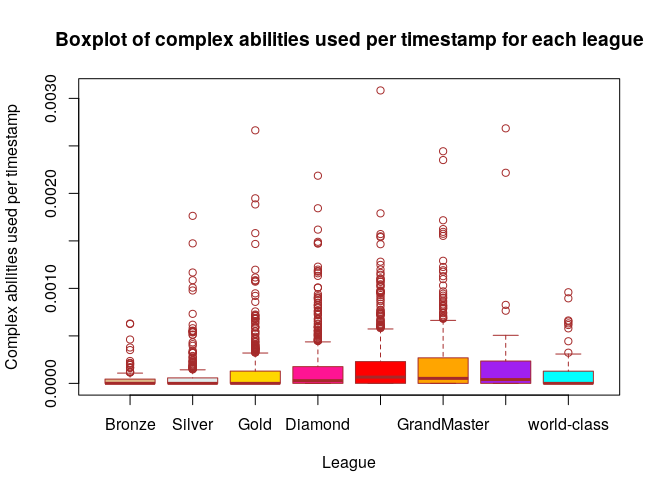
\includegraphics[width=0.8\textwidth]{abilities_boxplot.png}
    \label{figure:figure:abilities-boxplot}
    \caption{How often complex abilities are used per timestamp in each league.}
\end{figure}

\section{Analysis}
Before utilizing multivariate methods, let us form an hypothesis based on the information we have so far gained. In the APM to league boxplot (figure 1) there is a steady rise in APM as the leagues progress, which hint towards some degree of correlation there. Figure 2 depicts similar correlation for hotkey per timestamp for each league, although the rise is a bit less dramatic here. Complex abilities on the other hand seem to be quite evenly distributed with outliers excisting in almost every league. Based on this, the hypothesis is that APM and hotkey usage should correlate strongly with the league of the player and complex ability usage should not.

Figure 5 shows the pairwise relationships between each variable analyzed. This plot supports the hypothesis made, as we can see APM and selection by hotkeys rising as the league rises. This figure reveals the relationship between APM and selection by hotkeys: their shared plot is almost linear. This is an reasonable result, as using many hotkeys efficiently allows a player to perform more actions, meaning their APM rises. Complex ability usage does not contribute so clearly to a higher league, or correlate with the other variables. Players with a decent, mid-level APM seem to use most complex abilities, even more than professional players. Additional curiosity is revealed by the relationship between selection by hotkeys and complex abilities used: players that perform the least selections by hotkeys seem to use the most complex abilities.

\begin{figure}[H]
    \centering
    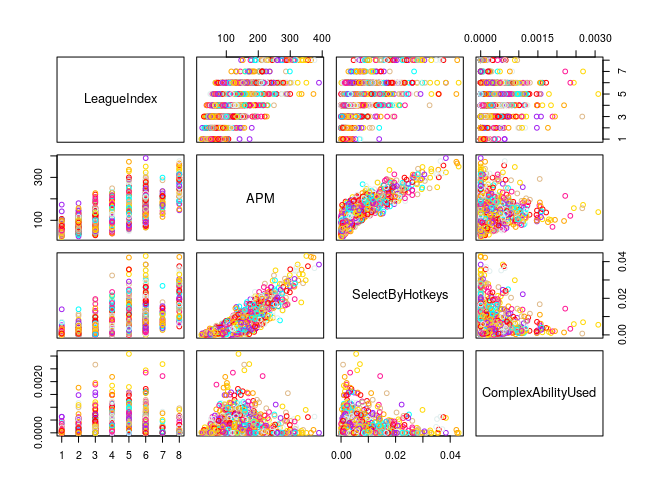
\includegraphics[width=\textwidth]{variables.png}
    \label{figure:variables}
    \caption{Scatterplot of all of the variables.}
\end{figure}

\subsection{Clustering}
To find correlations between the three variables and how they relate to the leagues introduced, clustering is applied. More specifically, k-means clustering is applied because of the quantitative nature of the data. Because of the growth of APM and hotkey usage as a player's league rises, clustering has a chance to succesfully classify each league correctly. We want to end up with as many clusters as there are leagues. When clustering was performed, the leagues were left out so that the clusters would not be affected by the "correct answers".

\begin{figure} [H]
    \centering
    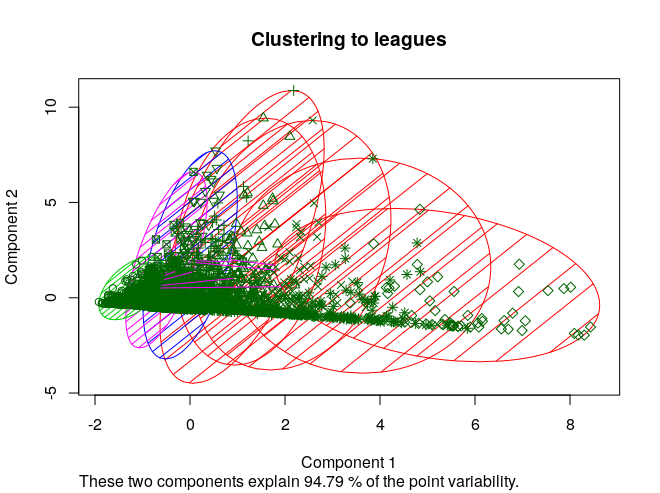
\includegraphics[width=\textwidth]{clustering.png}
    \label{figure:clustering}
    \caption{Results of applying k-means clustering to the dataset.}
\end{figure}

As can be seen from the results of clustering in figure 6, the clusters have a lot of overlap. The centers of the clusters are in a more or less straight line across the component one of the figure. This indicates that component one largely consists of APM, as it had by far the largest variance out of the variables. The huge overlap of the clusters indicates that way as well, since as we saw earlier, the APM increases as league increases but quite slowly and especially the middle leagues have many outliers.

\section{Conclusions}
Returning to the research questions introduced, yes, a players league can be predicted by observing their in-game behavior. But making an accurate prediction with the variables utilized is not trivial. If the target of a prediction is either a player in the lower leagues of bronze or silver, or in the professional leagues, the prediction has a good chance of matching the player's actual league. The middle ground between these two ends is harder to predict, as none of the three variables exhibits unique ranges of values for the leagues. Instead, the values have a lot of overlap between the leagues, making predictions hard. The results of applying clustering to the data support this result, as the clusters overlap extensively.

APM provides the best clues for the league of a player, as it rises steadily along with leagues. Hotkey usage rises as well, but not as fast and the leagues have a lot of outliers.

I chose to stick with the variables utilized because of my personal interest in how they would correlate with rankings and did not want to end up with too many variables to explain. A point of criticism is the amount of variables as additional ones were available and could have made for far better measures. Other multivariate analysis methods could have been utilized as well, instead of performing only clustering. The results felt quite clear, which is why I settled to using only clustering, but of course other methods could have revealed some curiosities.
\end{document}
